To demonstrate the performance of our lens modeling pipeline,
%code is consistent with existing codes, 
we simulate a sample of \agu{100} systems using \texttt{lenstronomy} (see \cref{fig:lens-sample}). 
The parameters for these systems are sampled from the simulation distribution defined in \cref{eqn:sim-dist}. \agu{Our prior, also defined in \cref{eqn:sim-dist}, has the same center as the simulation distribution, but has been broadened considerably so that it is less informative.}

%\ag{. However, this distribution is consistent with numbers reported in \citet{auger2010a} $\gamma$ and the lens half-light radius distribution.}

%\begin{figure}[ht]
\begin{minipage}{0.96\linewidth}
%\begin{center}
\vspace{1mm}
\makebox[\linewidth]{
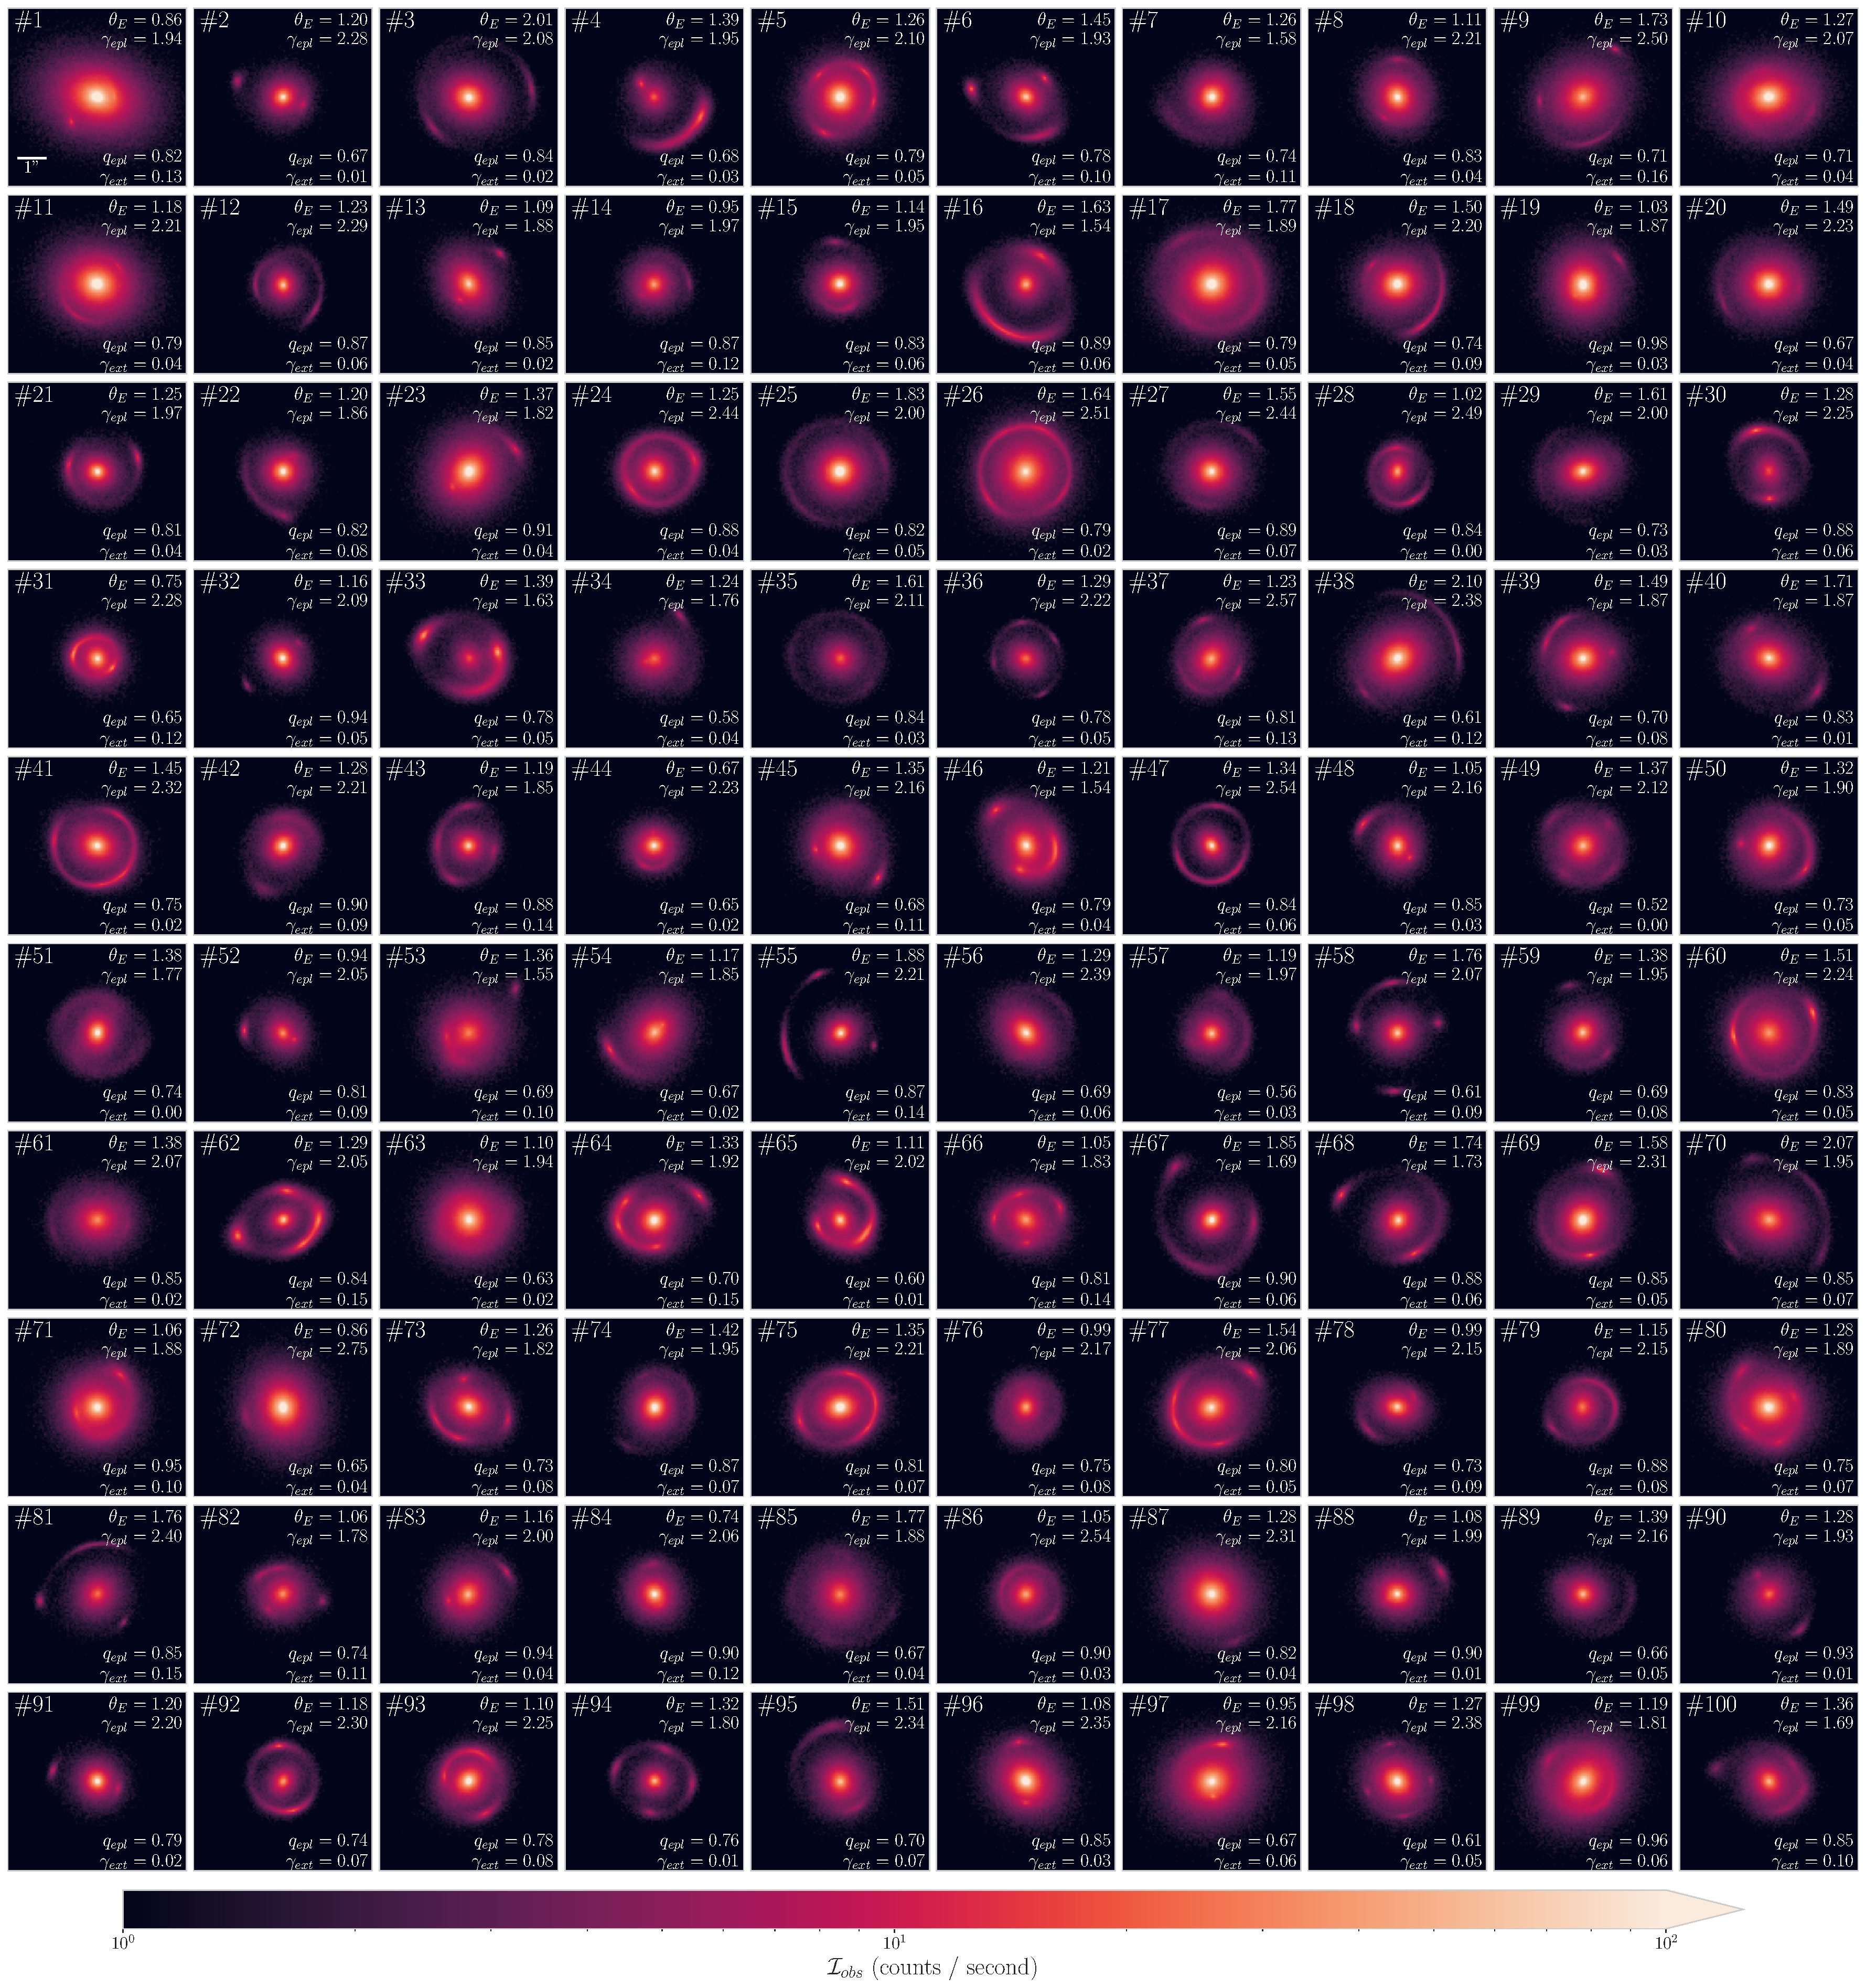
\includegraphics[width=\textwidth]{figures/lens_sample.pdf}}
    \captionof{figure}
    {%\vspace{-50mm} 
    A sample of \agu{100} lenses simulated using \texttt{lenstronomy}. We include the effects of Gaussian noise with standard deviation $\sigma_{bkg}=0.2$, Poisson shot noise with an exposure time $t_{exp}=100 \ \text{sec}$ with $\mathcal{G}=1$ \aguu{(assuming \hst observations)}, and the PSF (see \cref{fig:ref-sys}). \agu{The pixel scale is $0.065\twopr$ and the cutout size is $5.2\twopr \times 5.2 \twopr$ (80 pixels by 80 pixels).}}
    \label{fig:lens-sample}    
%\end{center}
\vspace{2mm}
\end{minipage}

We apply our modeling pipeline as described in \cref{tab:pipeline} to each of these systems and show the excellent agreement with \agu{the ground truth} (input values) in \cref{fig:sim-parity}. \agu{The hyperparameters listed in \cref{tab:pipeline} were roughly tuned (to the appropriate order of magnitude) on the reference system, and left unchanged when modeling the sample of 100 simulated systems.} \ag{The average time to model one simulated system is comparable to the reference system  \aguu{(see \cref{tab:pipeline})}.}
%The close agreement indicates our lensing code is consistent with \texttt{lenstronomy}. 
Moreover, we find that our pipeline consistently exhibits favorable MC convergence (\cref{tab:err}): even the largest $\hat{R}$ for any parameter over all \agu{100} simulated systems was $1.017$, and the smallest ESS was $26822$, an order of magnitude higher than the typical value with \emcee.
%For comparison, recall that on the reference system (\cref{fig:ref-sys}) using the same number of MCMC walkers and iterations with \texttt{lenstronomy}, we find $\hat{R}$ is typically $1.5$, $ESS$ is typically $\sim 100$.


\begin{minipage}{0.96\linewidth}
%\vspace{-2mm}
%\begin{center}
\makebox[\linewidth]{
    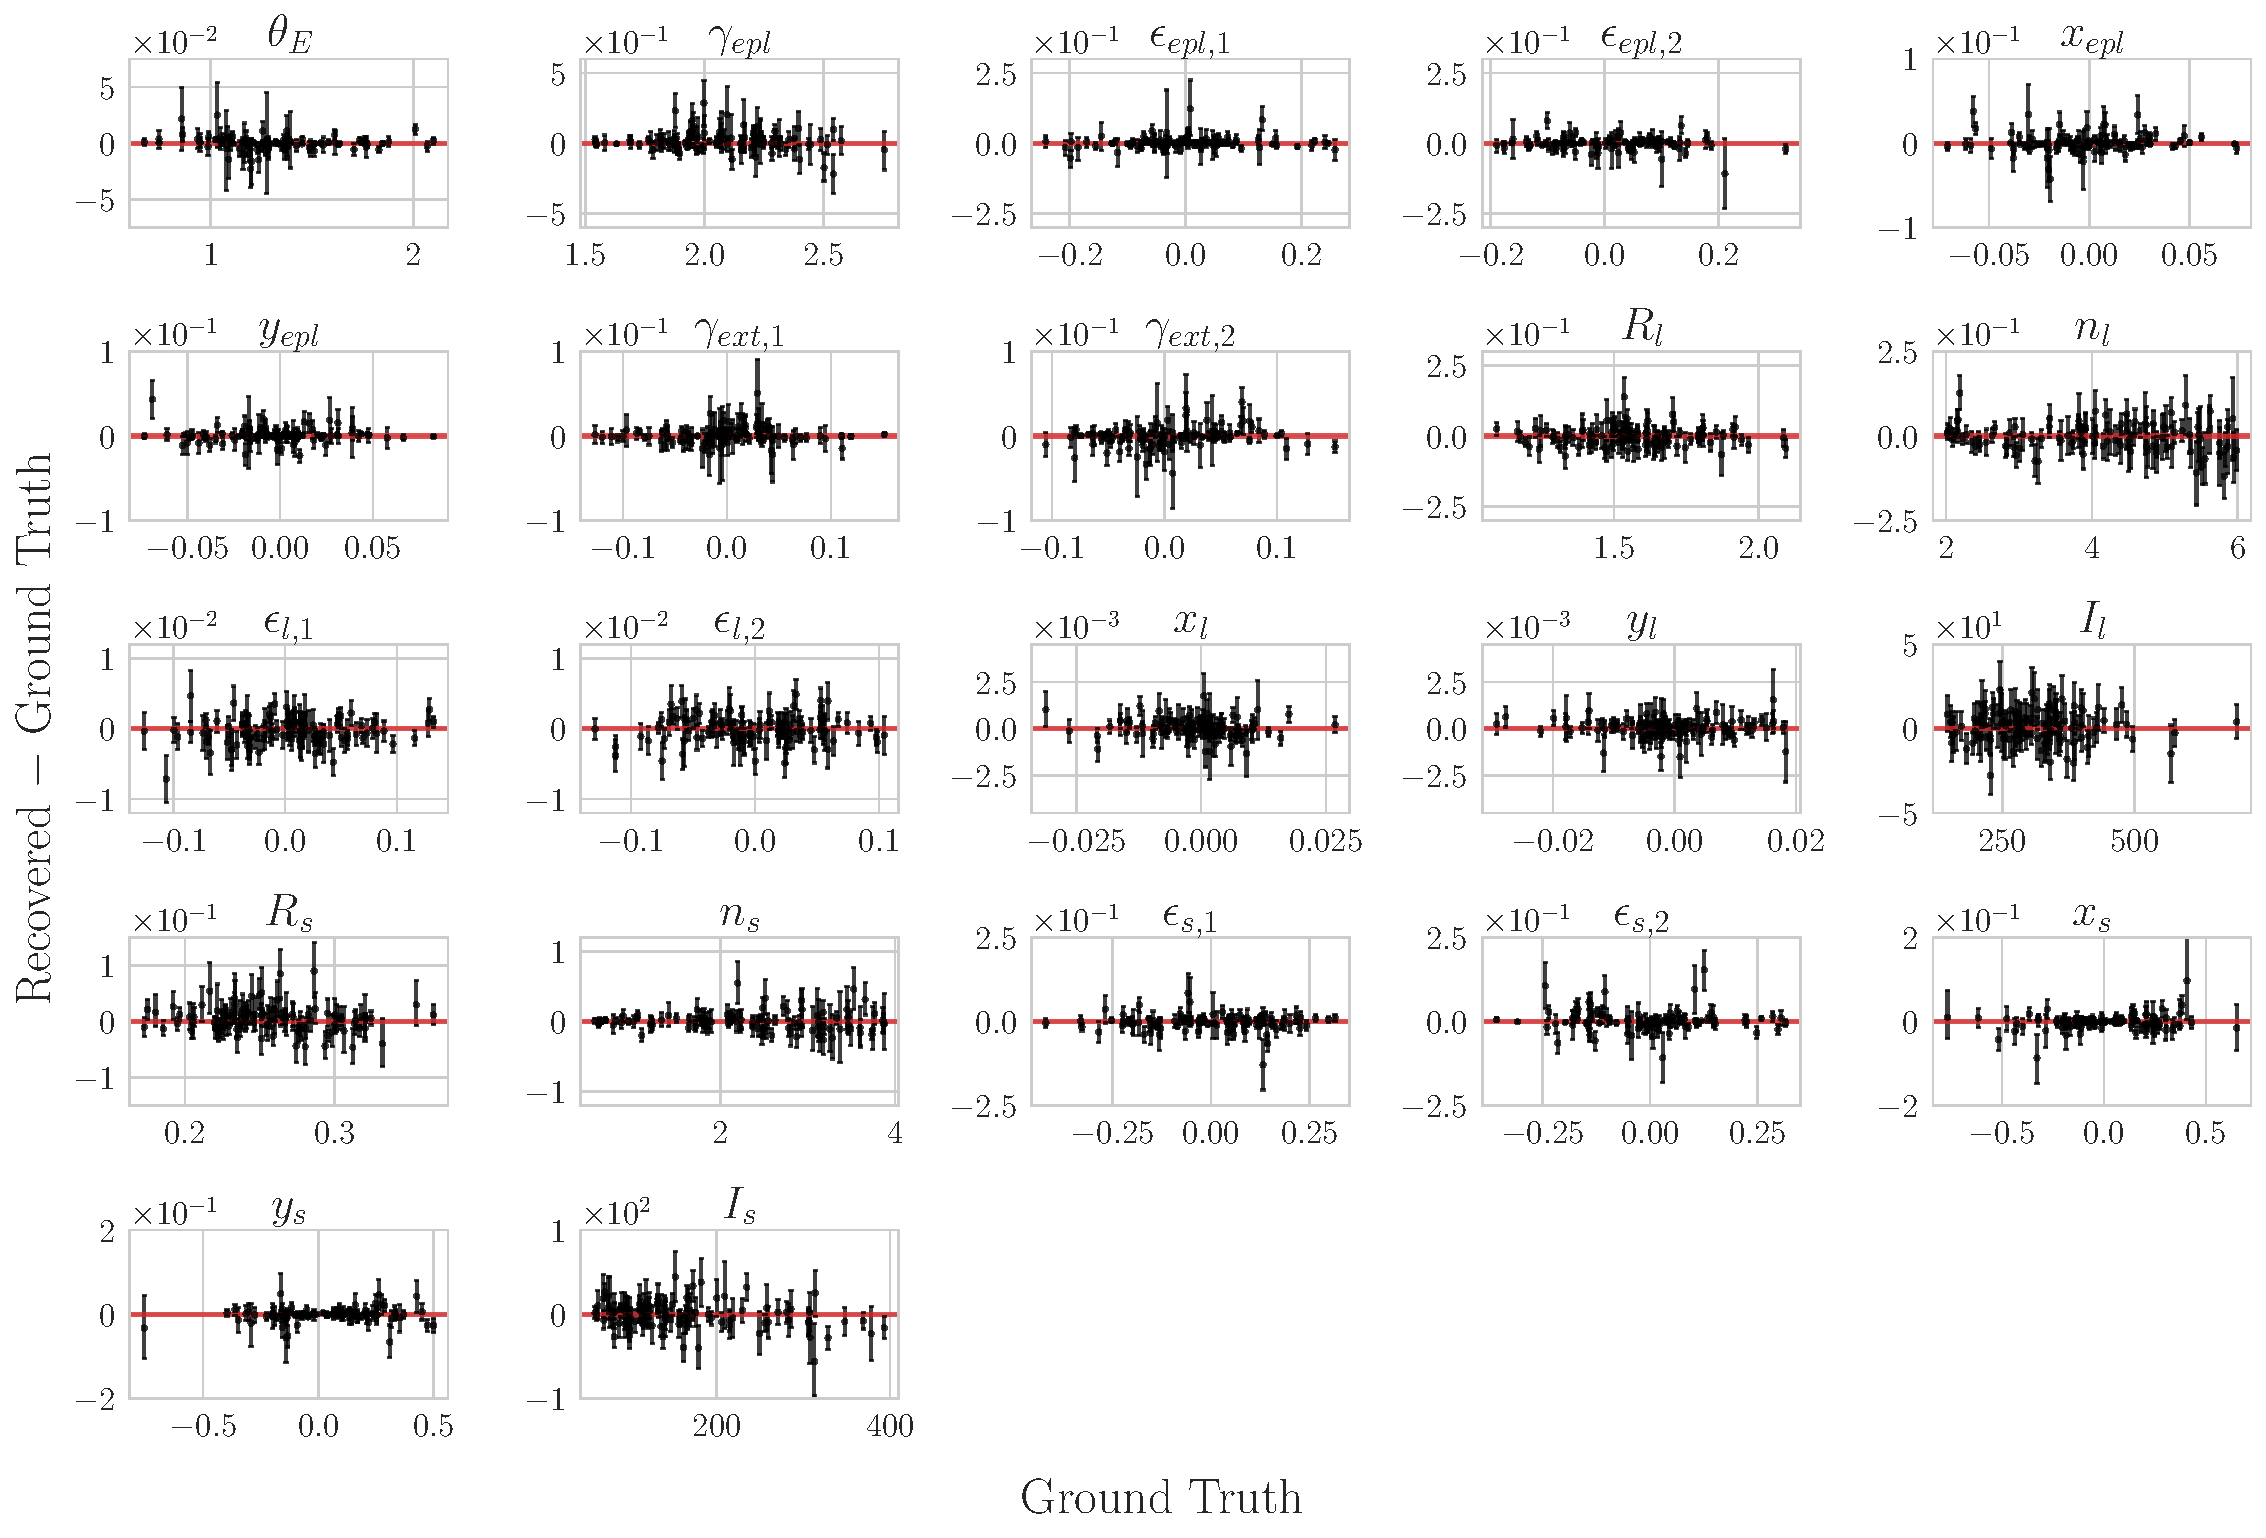
\includegraphics[width=\textwidth]{figures/sim-parity.pdf}}
    \captionof{figure}{Difference between the \ag{recovered parameters and} \agu{ground truth (input values)} for the \agu{100} simulated systems in \cref{fig:lens-sample}. The points are the mean of the posterior, and the uncertainties correspond to the 68\% highest posterior density interval. \agu{Note that as $n_l$ and $n_s$ increase, their uncertainties increase as well. This is because the light becomes more compact at higher S\'ersic indices, resulting in higher degeneracy between the S\'ersic indices and the half-light radii.}}
    \label{fig:sim-parity}
%\end{center}
\end{minipage}
%\input{multicol}

\begin{deluxetable}{lRR|RRRR}[H]
\tablecaption{Summary statistics of lensing parameters\label{tab:err}}
\tablehead{\colhead{Parameter} & \colhead{Mean error} & \colhead{$\mu_z$} & \colhead{$\langle \hat{R} \rangle$} & \colhead{$\max \hat{R}$} & \colhead{$\langle ESS \rangle$} & \colhead{$\min ESS$}}
\startdata
 $\bm{\theta_E}$ &    -0.00026 & -0.04 \pm 0.09 &                      1.001 &            1.013 &                  35465 &        30846 \\
    $\bm{\gamma_{epl}}$ &     0.01608 &  0.12 \pm 0.08 &                      1.001 &            1.017 &                  35407 &        28045 \\
$\bm{\epsilon_{epl,1}}$ &     0.00235 &  0.08 \pm 0.09 &                      1.001 &            1.011 &                  35590 &        29438 \\
$\bm{\epsilon_{epl,2}}$ &    -0.00159 &  0.01 \pm 0.10 &                      1.001 &            1.006 &                  35505 &        31213 \\
         $\bm{x_{epl}}$ &     0.00031 & -0.10 \pm 0.10 &                      1.001 &            1.004 &                  35617 &        33434 \\
         $\bm{y_{epl}}$ &     0.00082 &  0.06 \pm 0.09 &                      1.001 &            1.008 &                  35569 &        32745 \\
  $\bm{\gamma_{ext,1}}$ &     0.00088 &  0.07 \pm 0.09 &                      1.001 &            1.012 &                  35542 &        27926 \\
  $\bm{\gamma_{ext,2}}$ &    -0.00060 & -0.06 \pm 0.09 &                      1.001 &            1.010 &                  35382 &        30456 \\
             $\bm{R_l}$ &    -0.00203 & -0.09 \pm 0.09 &                      1.000 &            1.007 &                  35768 &        33695 \\
             $\bm{n_l}$ &    -0.00321 & -0.05 \pm 0.08 &                      1.000 &            1.008 &                  35777 &        33752 \\
  $\bm{\epsilon_{l,1}}$ &    -0.00038 & -0.21 \pm 0.10 &                      1.000 &            1.003 &                  35444 &        33593 \\
  $\bm{\epsilon_{l,2}}$ &    -0.00006 & -0.01 \pm 0.10 &                      1.001 &            1.003 &                  35495 &        33247 \\
             $\bm{x_l}$ &     0.00003 &  0.03 \pm 0.09 &                      1.001 &            1.003 &                  35687 &        33086 \\
             $\bm{y_l}$ &     0.00006 &  0.13 \pm 0.08 &                      1.000 &            1.003 &                  35641 &        32861 \\
             \aguu{$\bm{I_l}$} &     1.20330 &  0.07 \pm 0.08 &                      1.000 &            1.007 &                  35758 &        33603 \\
             $\bm{R_s}$ &     0.00599 &  0.13 \pm 0.09 &                      1.000 &            1.005 &                  35497 &        32109 \\
             $\bm{n_s}$ &     0.01192 &  0.04 \pm 0.09 &                      1.000 &            1.005 &                  35613 &        32820 \\
  $\bm{\epsilon_{s,1}}$ &    -0.00255 & -0.09 \pm 0.10 &                      1.000 &            1.004 &                  35556 &        31342 \\
  $\bm{\epsilon_{s,2}}$ &     0.00282 &  0.05 \pm 0.10 &                      1.001 &            1.005 &                  35711 &        31810 \\
             $\bm{x_s}$ &    -0.00087 & -0.06 \pm 0.09 &                      1.001 &            1.017 &                  35443 &        26822 \\
             $\bm{y_s}$ &    -0.00092 &  0.03 \pm 0.08 &                      1.001 &            1.017 &                  35470 &        29876 \\
             \aguu{$\bm{I_s}$} &    -0.09109 & -0.05 \pm 0.09 &                      1.000 &            1.003 &                  35580 &        33416
\enddata
\tablecomments{We show the errors for the 22 lensing parameters in \cref{fig:sim-parity}. Mean error denotes the average difference between the recovered parameters and the \agu{ground truth} for the \agu{100} simulated systems.
The notation $z$ denotes errors that have been scaled by the posterior standard deviation. \agu{For example, for a given system, if the posterior mean and variance of the Einstein radius are $\mathbb{E}[\theta_E],\mathbb{V}[\theta_E]$, and the ground truth Einstein radius is $\bar{\theta}_E$, then $z[\theta_E]=(\mathbb{E}[\theta_E]-\bar{\theta}_E)/\sqrt{\mathbb{V}[\theta_E]}$. We report the average (over all 100 systems) scaled error $\mu_z$ for each parameter, and find that they are all consistent with zero bias.} We also report statistics for the MC convergence diagnostics, including the mean and extremal values. Specifically, for any given parameter, the $\max \hat{R}$ and $\min ESS$ values are the largest $\hat{R}$ and smallest $ESS$ for that parameter across all \agu{100} simulated systems.}
\end{deluxetable}

% \subsection{Demonstration on an HST Observed System}\label{sec:result-ray-obs}
% We apply our modeling pipeline to an observed HST system, and show that it is well-suited for efficient inference on complex models. We preprocess the data by drizzling three exposures to $0.065"$, and estimate the background noise level $\sigma_{bkg}$ with \texttt{photutils} \citep{larry2020}. The PSF (shown in \cref{fig:ref-sys}) is modeled using \texttt{TinyTim} with a late-type galaxy spectral template, obtained from SDSS-DR6. Our prior is:
% \begin{align}
% \begin{split}\label{eqn:hst-sim-dist}
% \text{Lens}: &
% \left\lbrace
% \array{@{}r@{\quad}l@{}r@{}}%
% \theta_{E}& \sim \exp(\mathcal{N}(\ln 1.2, 0.5)) & \text{[Einstein radius, in arcseconds]} \\
% \gamma_{epl} &\sim \mathcal{N}(2, 0.30) & \text{[Mass slope]} \\
% \epsilon_{1, epl}, \epsilon_{2, epl} &\sim \mathcal{N}(0, 0.15) &
% \text{[Lens mass profile complex ellipticity]} \\
% x_{epl}, y_{epl} &\sim \mathcal{N}(0, 0.05) & \text{[Lens center, in arcseconds]} \\
% \gamma_{1, ext}, \gamma_{2, ext} \qquad &\sim \mathcal{N}(0, 0.05) & \text{[External shear components]}
% \endarray \right. \\
% \text{Lens Light}: &
% \left\lbrace
% \array{@{}r@{\quad}l@{}r@{}}%
% R_{lens}[i] &\sim \exp(\mathcal{N}(\ln 1, 0.7)) & \text{\qquad\quad [S\'ersic radius, in arcseconds]} \\
% n_{lens}[i] &\sim \mathcal{U}(0, 10) & \text{[S\'ersic index]} \\
% \epsilon_{1, src}[i], \epsilon_{2, src}[i] &\sim \mathcal{N}(0, 0.3) & \text{[Lens light complex ellipticity]}\\
% x_{lens}[i], y_{lens}[i] &\sim \mathcal{N}(0, 0.05) & \text{[Lens light center, in arcseconds]}
% \endarray \right. \\
% \text{Source Light}: &\left\lbrace
% \array{@{}r@{\quad}l@{}r@{}}%
% R_{src}[i] &\sim \exp(\mathcal{N}(\ln 0.2, 0.2)) & \text{[S\'ersic radius, in arcseconds]} \\
% n_{src}[i] &\sim \mathcal{U}(0, 10) & \text{[S\'ersic index]} \\
% \epsilon_{1, src}[i], \epsilon_{2, src}[i] &\sim \mathcal{N}(0, 0.3) & \text{[Source light complex ellipticity]}\\
% x_{src}[i], y_{src}[i] &\sim \mathcal{N}(0, 0.5) & \text{[Source light center, in arcseconds]}
% \endarray \right.
% \end{split}
% \end{align}
% Our system cutout is chosen such that the brightest pixel of the lens light is at the center of the image. Previous work has found that S\'ersic profiles do not fit lens light well near the center of the lens \citep{shajib2021}, and therefore a small disc with a $0.26"$ radius is masked out from the center of the lens light \citep[as done in][]{shajib2021}. A small interloper in the southeast corner of the image is also masked out with a $0.65" \times 0.65"$ square. We show modeling results using three elliptical S\'ersic components for the source (\cref{fig:hst-3src}) and two S\'ersic components to model the lens light. 

% \begin{figure}
%     \centering
%     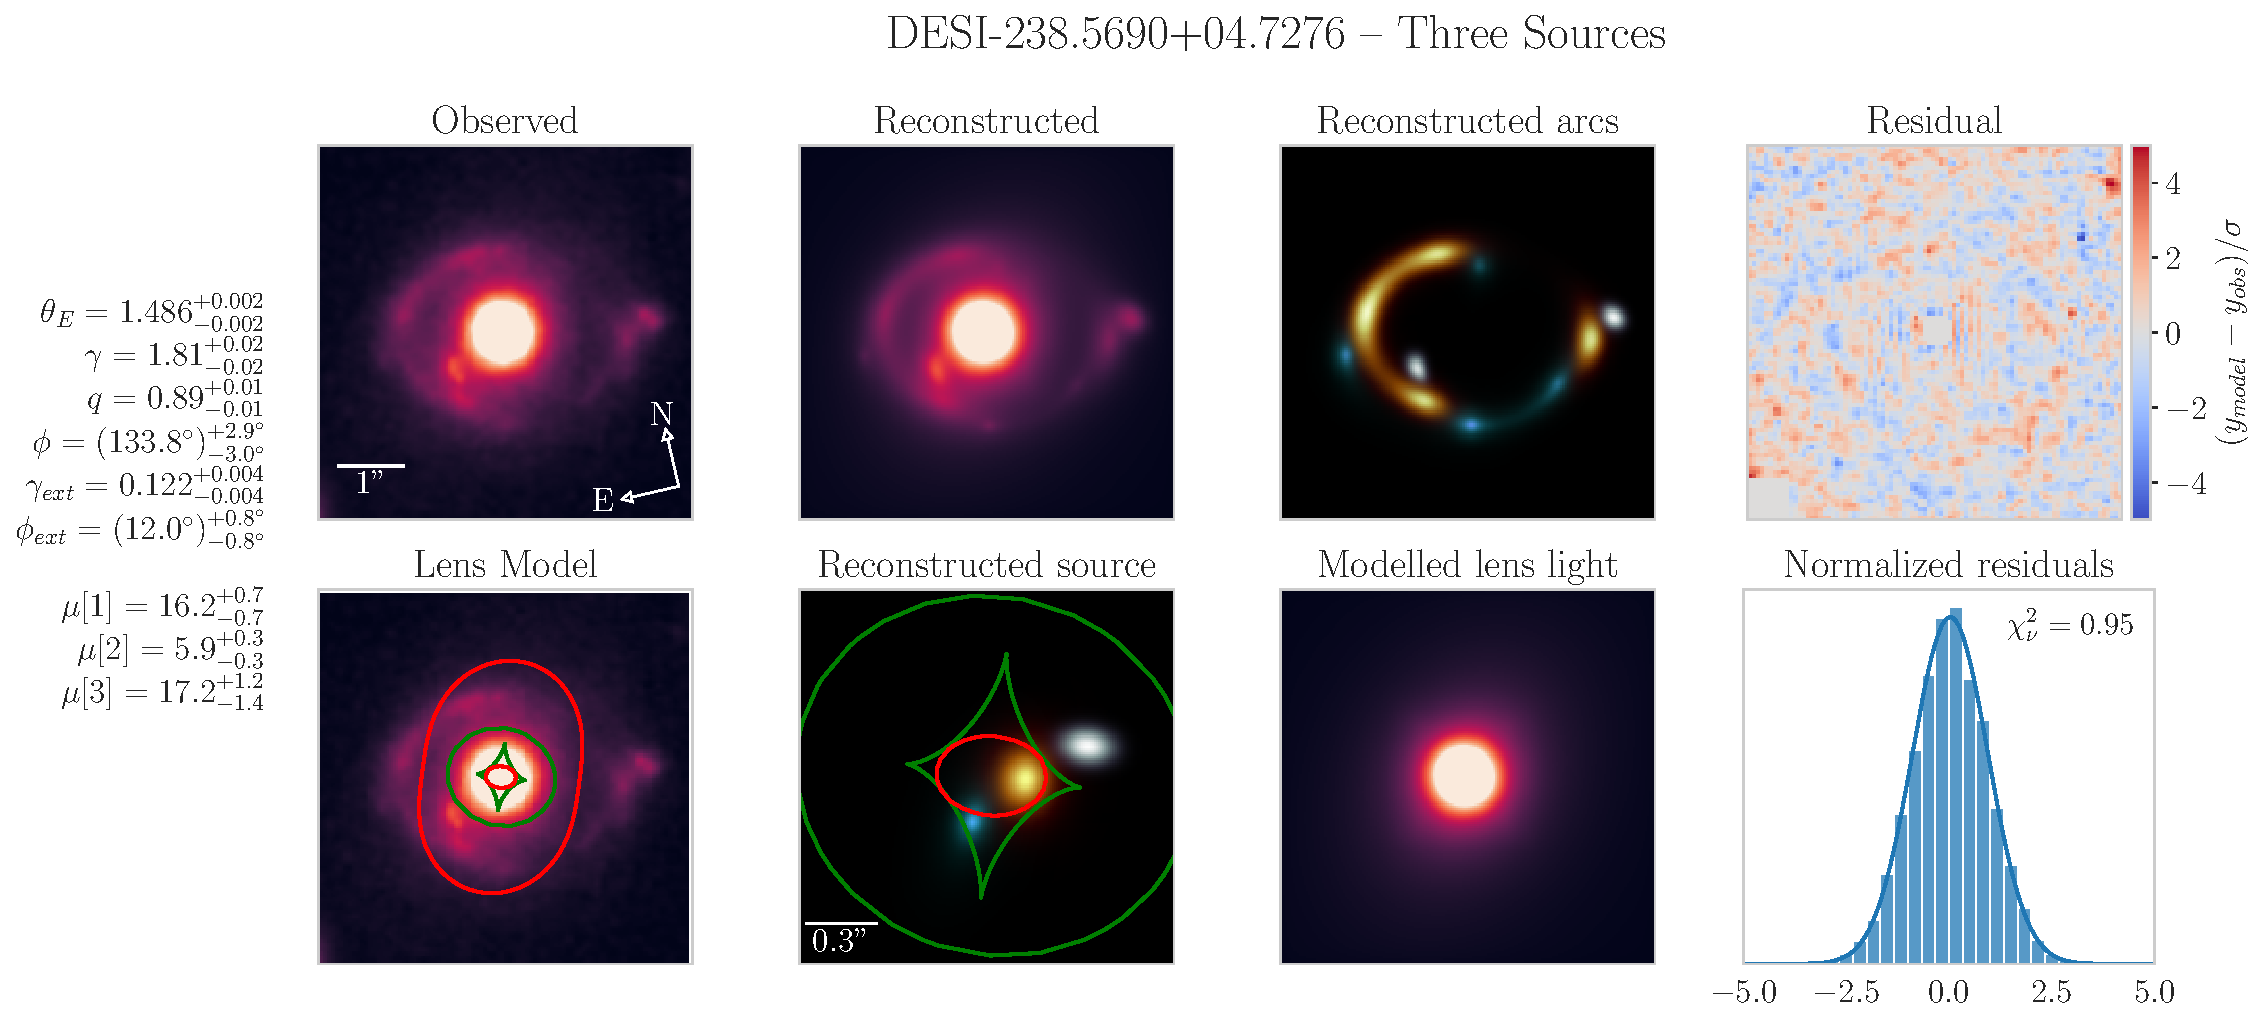
\includegraphics[width=\textwidth]{figures/hst-3src.pdf}
%     \caption{Modeling results for \sysname \ with three elliptical S\'ersic components in the source plane. The three sources are shown in false color: the copper source corresponds to $i=1$, the blue-white corresponds to $i=2$, and the pink corresponds to $i=3$.}
%     \label{fig:hst-3src}
% \end{figure}


% \begin{figure}
%     \centering
%     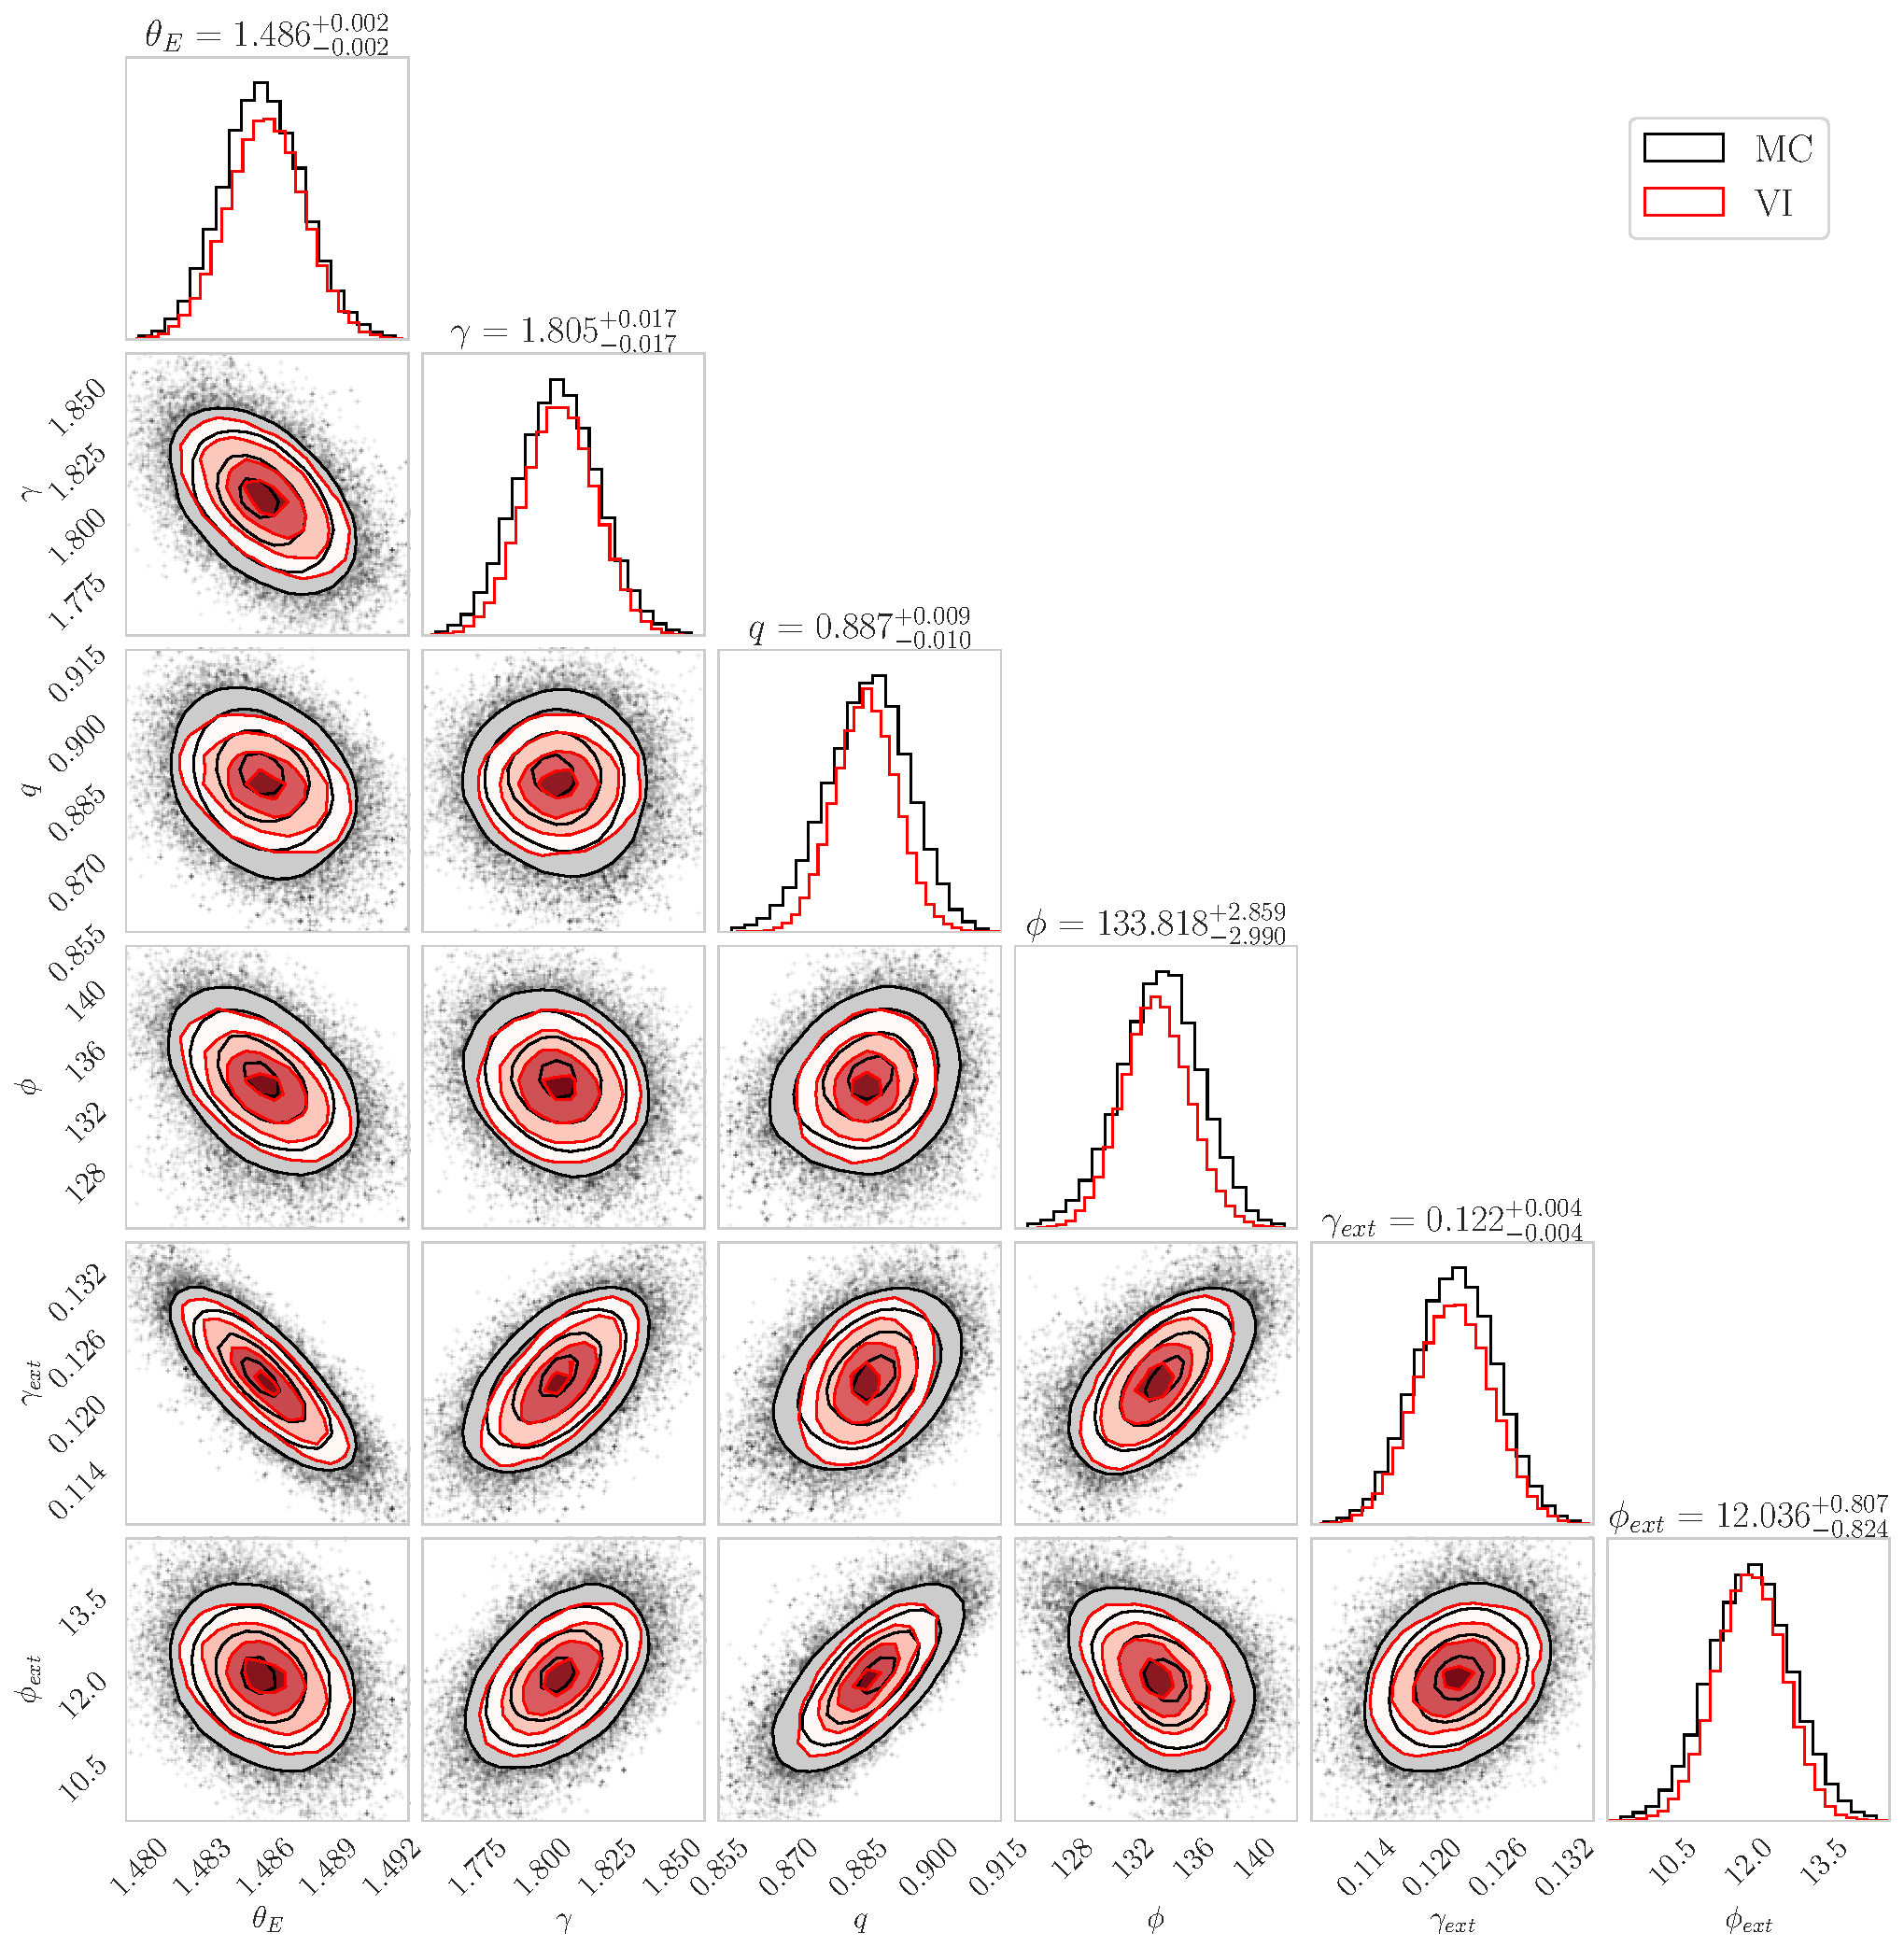
\includegraphics[width=0.8\textwidth]{figures/hst-3src-corner.pdf}
%     \caption{Samples drawn from HMC and VI for \sysname. The VI samples exhibit non-Gaussianity for certain parameters (i.e., $\phi,\phi_{ext}$) because these variables are non-linear transformations of the inferred VI parameters $\epsilon_1,\epsilon_2$ and $\gamma_1,\gamma_2$. We also point out the close agreement between the surrogate posterior inferred via VI and the HMC samples.}
%     \label{fig:hst-3src-corner}
% \end{figure}

% \begin{figure}
%     \centering
%     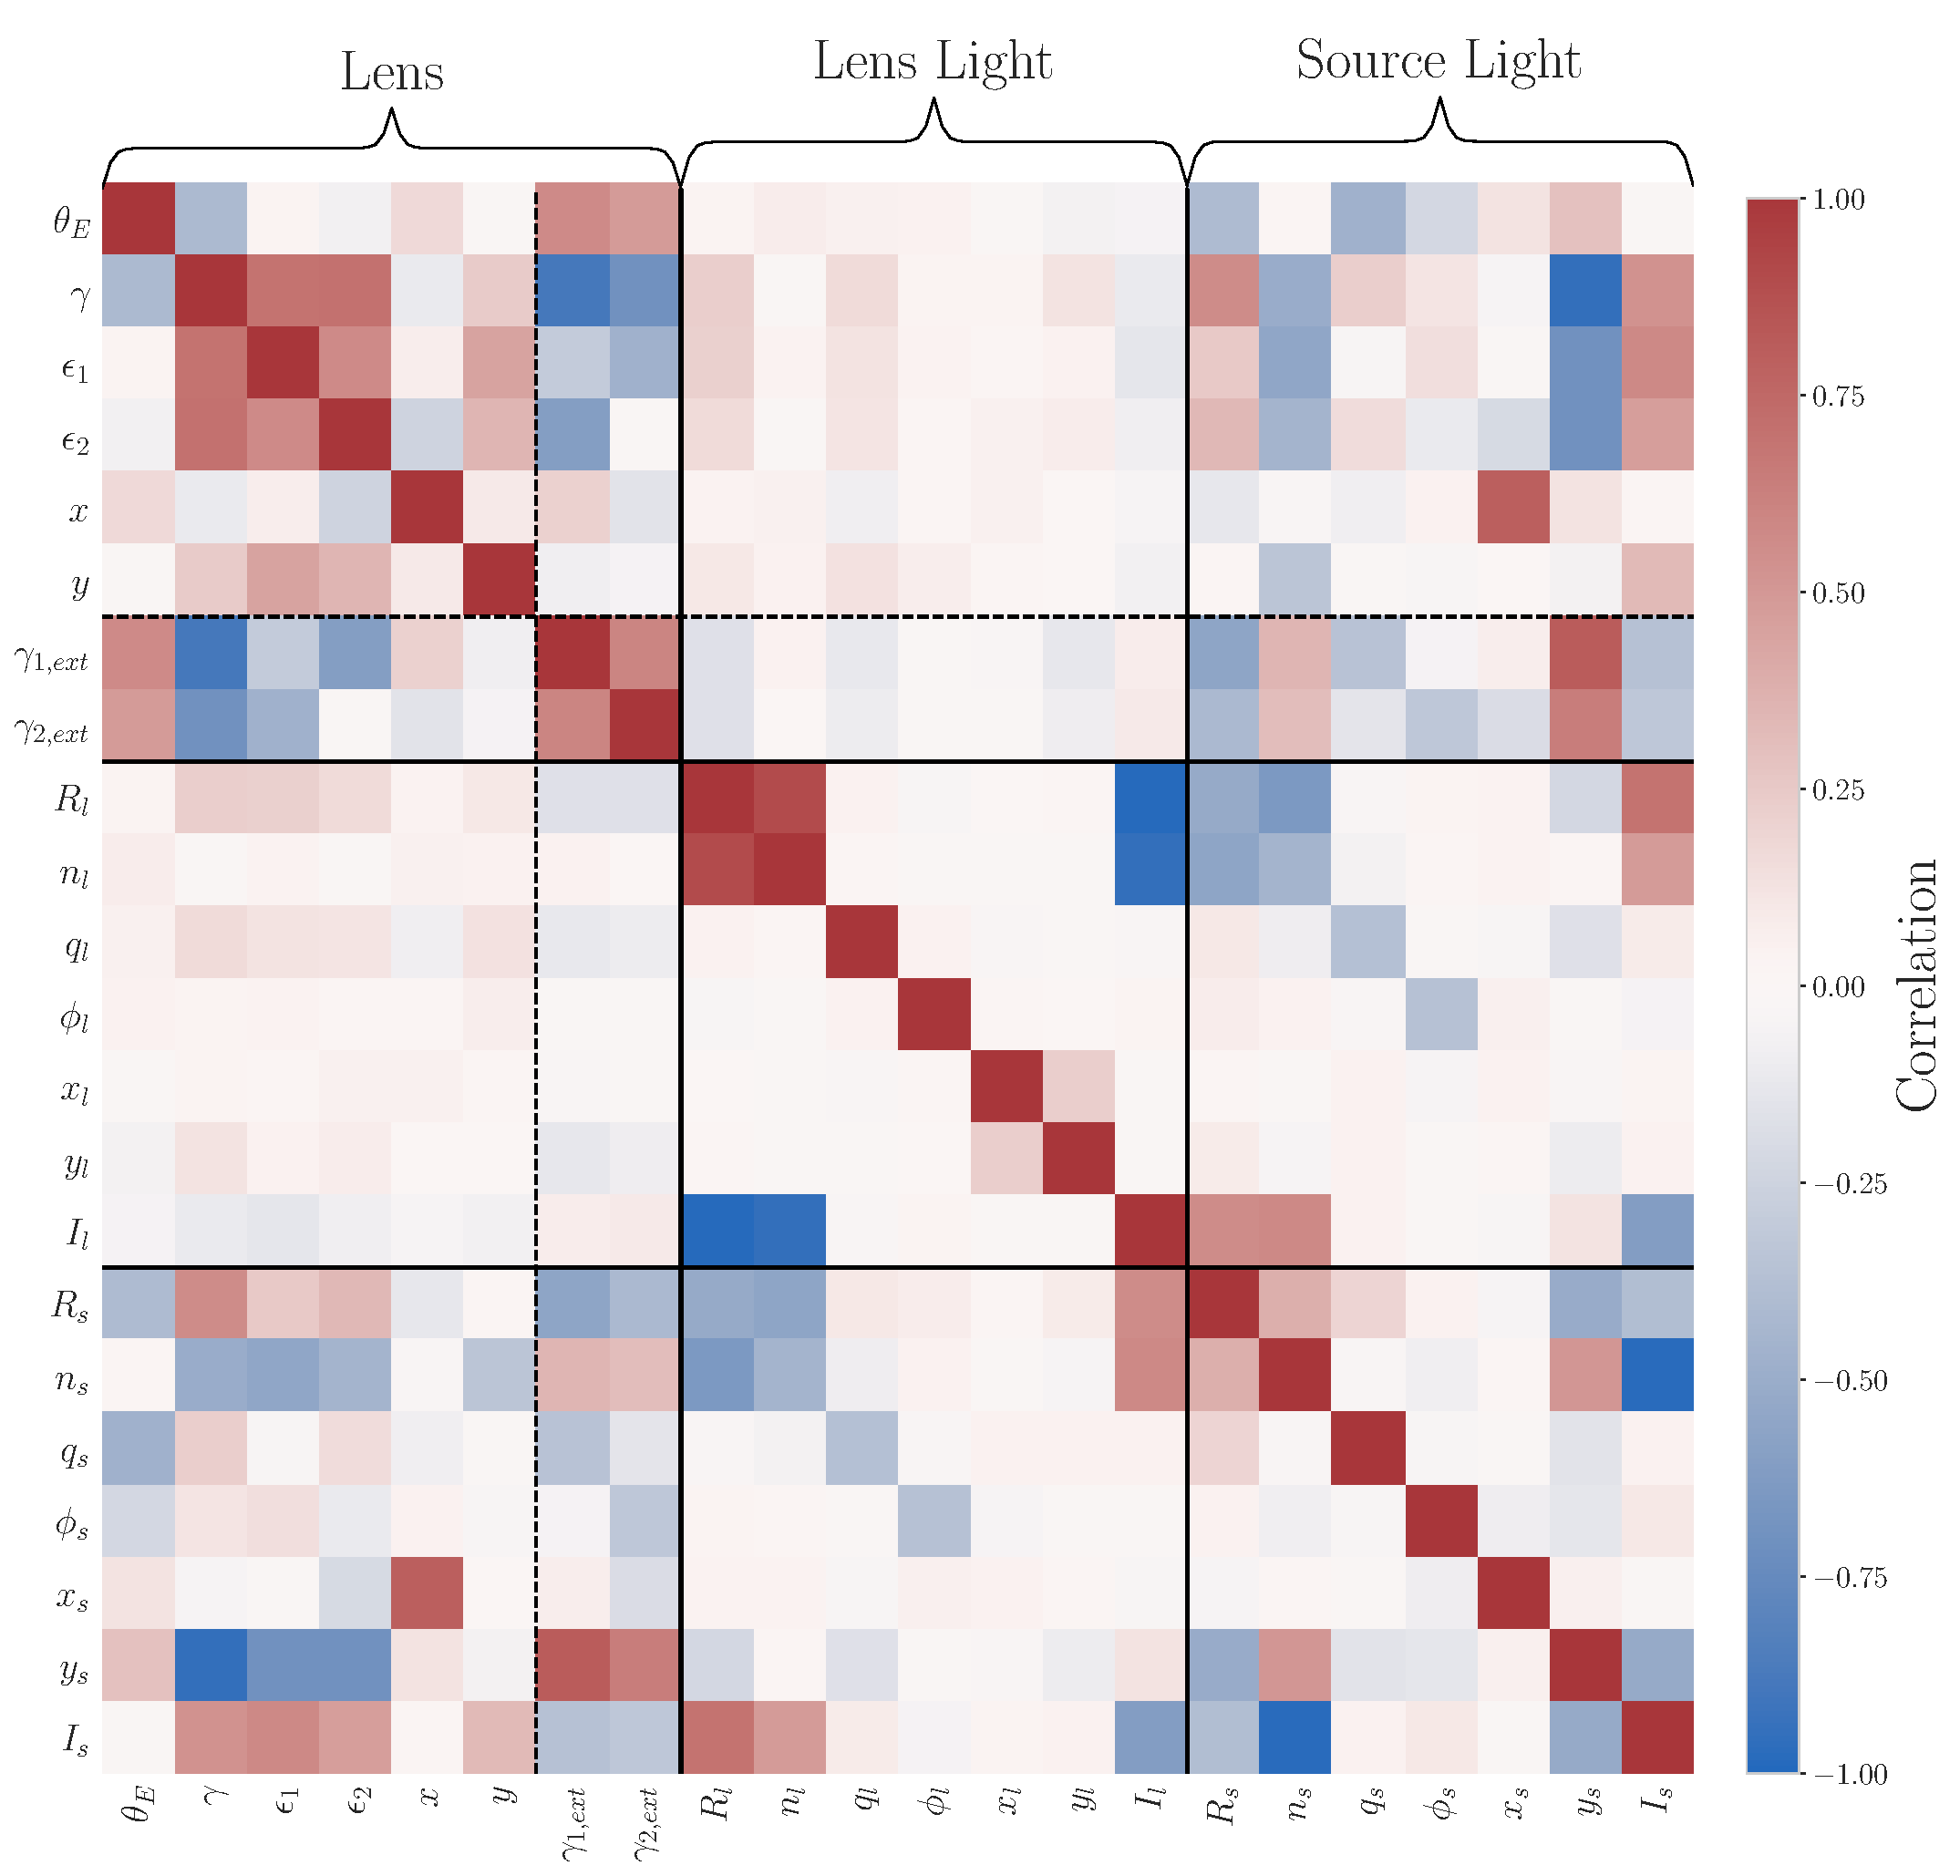
\includegraphics[width=0.9\textwidth]{figures/hst-3src-corr.pdf}
%     \caption{The correlation matrix for the posterior distribution of \sysname. Note the absence of correlation between lens light and lens parameters, compared against the presence of strong correlations between source light and lens parameters.}
%     \label{fig:hst-3src-corr}
% \end{figure}